\newpage
\section{Resultate}
\subsection{Zielerreichung}
Das Projekt OSM Crosswalk Detection barg einige Hürden, von der Schwierigkeit der Bilderkennung, dem Anbinden diverser Schnittstellen und die parallele Verarbeitung grosser Datenmengen.\\
Als Resultat der Arbeit entstand eine Applikation, welche auf Orthofotos Fussgängerstreifen erkennt und deren Koordinaten speichert. Im Bild unterhalb sind die vom Algorithmus gefundenen Fussgängerstreifen der Ostschweiz visualisiert. \\
\begin{figure}[H]
\centering
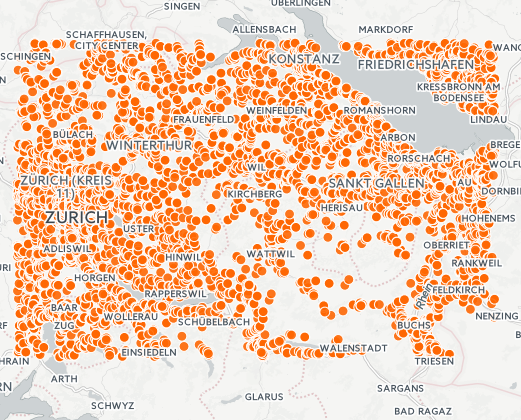
\includegraphics[width=350pt]{images/ostschweiz.png}
\caption[Ostschweiz]{Ostschweiz}
\end{figure}

\subsubsection{Confusion Matrix}
Um saubere Kennzahlen zur Erkennungrate zu erhalten, haben den Algortihmus auf die Fläche zwischen Zollikon und Zürich Zoo angewendet und die Daten in einer Confusion Matrix zusammengefasst.
\\
\begin{figure}[H]
	\centering
	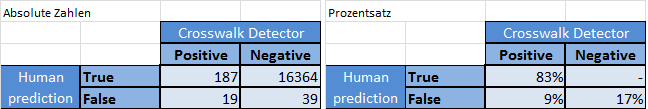
\includegraphics[]{images/Confusionmatrix_dl_end.png}
	\caption[Resultierende Confusion Matrix]{Resultierende Confusion Matrix - BBox (47.355633, 8.543026), (47.372811, 8.570957)}
\end{figure}
In Worten ausgedrückt, sind die Zahlen folgendermassen zu interpretieren:
\begin{itemize}
	\item 83\% aller visuell sichtbaren Fussgängerstreifen werden erkannt.
	\item 17\% der Fussgängerstreifen werden nicht erkannt.
	\item 9\% der erkannten Fussgängerstreifen sind falsch.
\end{itemize}
			


\subsubsection{Ziel der Aufgabenstellung}
\begin{table}[H]
    \begin{tabular}{|p{6cm}|p{8cm}|}
    \hline    
    \rowcolor{lightblue}
	Ziel & Resultat \\ \hline
	Evaluation eines effizienten Algorithmus zur Erkennung von Fussgängerstreifen auf Orthofotos. & Diverse Algorithmen wurden evaluiert, mit dem Deep Learning Ansatz wurde ein klarer Favorit ermittelt. Mehr dazu unter dem Abschnitt~\ref{sec:suchalgorithmus} auf der Seite~\pageref{sec:suchalgorithmus}.\\ \hline
	Automatische Verarbeitung von Orthofotos. & Es wird automatisch auf Bilder von Bing Maps zugegriffen.\\ \hline
	Extraktion der Koordinaten von Fussgängerstreifen aus Orthofotos (Kanton Zürich, optional Europa oder mehr). & Zürich konnte von der Applikation verarbeitet werden, weiter wurde die Suche auf die Ostschweiz ausgebaut. \\ \hline
	Evaluation des Crowdsourcing-System zur Daten-Validierung und Übertragung in OSM.& Bei der Evaluation des Crowdsourcing-Systems setzte sich MapRoulette durch die Bekanntschaft bei der Community durch. Mehr dazu unter dem Abschnitt~\ref{sec:crowdsourcing} auf der Seite~\pageref{sec:crowdsourcing}. \\ \hline
	Erstellung einer Challenge für das Crowdsourcing-System anhand der gesammelten Daten. & Eine Challenge wurde für MapRoulette generiert und publiziert.\\ \hline
    \end{tabular}
    \caption[Resultate]{Resultate}
\end{table}
Die in der Aufgabenstellung formulierten Ziele konnten alle in einem angemessenem Rahmen erreicht werden. 

\newpage
\subsection{Persönlicher Bericht}
Mit dem Resultat des Projektes sind wir äusserst zufrieden. Es wurde viel neues dazugelernt, sowohl in technischen Bereichen, wie auch in der Teamkommunikation und dem Projektmanagement.
\subsubsection{Neu erlernte Technologien}
\begin{itemize}
	\item Python
	\item Docker
	\item Anwendung Neuronale Netze (Keras)
	\item OpenCV
\end{itemize}

\subsubsection{Daten}
Weiter hatten wir es mit einer grossen Datenmenge zu tun. In Zahlen gesprochen:
\begin{tabbing}
    \hspace*{8cm}\=\hspace*{4cm}\= \kill
    Durchsuchte Fläche: \> $8800 km^{2}$  \\
    Anzahl Tiles: \> 1'512'028 (à $5820 m^{2}$ pro Tile)\\
\end{tabbing}
Einerseits stellte die Datenbeschaffung schon ein grosse Herausforderung dar, andererseits war auch die parallele Verarbeitung nicht trivial. Mit der Queueing Lösung konnten wir dem jedoch erfolgreich entgegenwirken.
\newpage
\subsection{Dank}
Für die Betreuung während des ganzen Projektes möchten wir uns besonders bei Herr Prof. Stefan Keller Bedanken, der immer ein offenes Ohr für Problem aller Art hatte und uns freien Spielraum für die Suche nach einer optimalen Lösung gewährte. \\
Weiter geht auch ein Dank an Herr Prof. Dr.  Guido Schuster, welcher uns in Bezug auf den Erkennungsalgorithmus unterstützte. \\
Nicht zu vergessen sind die Mitarbeiter des Geometalabs (Teil des Institut für Software der HSR), welche uns bei der Findung einer passenden Lösung für die parallele Verarbeitung der Daten halfen.\\
Und zu guter Letzt möchten wir auch noch Manuel Roth und Lukas Martinell Danken, die uns in Fragen rund um Tiles und deren Umrechnung unterstützten.
	
